\documentclass[
% -- opções da classe memoir --
article,			% indica que é um artigo acadêmico
12pt,				% tamanho da fonte
oneside,			% para impressão apenas no recto. Oposto a twoside
a4paper,			% tamanho do papel. 
english,			% idioma adicional para hifenização
brazil,				% o último idioma é o principal do documento
sumario=tradicional
]{abntex2}
% ---
% PACOTES
% ---
\usepackage{lmodern} % Usa a fonte Latin Modern
\usepackage[T1]{fontenc}% Selecao de codigos de fonte.
\usepackage[utf8]{inputenc}% Codificacao do documento (conversão automática dos acentos)
\usepackage{indentfirst}% Indenta o primeiro parágrafo de cada seção.
\usepackage{nomencl} % Lista de simbolos
\usepackage{color}% Controle das cores
\usepackage{graphicx}% Inclusão de gráficos
\usepackage{microtype}% para melhorias de justificação
\usepackage{gensymb}
\usepackage{caption}
\usepackage{booktabs}
\usepackage{footnote}

% ---
% Pacotes adicionais, usados apenas no âmbito do Modelo Canônico do abnteX2
% ---
% ---
% Pacotes de citações
% ---
\usepackage[brazilian,hyperpageref]{backref}	 % Paginas com as citações na bibl
%\usepackage[alf,abnt-emphasize=bf]{abntex2cite}	% Citações padrão ABNT
\usepackage[num,overcite,abnt-emphasize=bf]{abntex2cite}	% Citações padrão ABNT
%\citebrackets()
\citebrackets[]
% ---

% ---
% Configurações do pacote backref
% Usado sem a opção hyperpageref de backref
\renewcommand{\backrefpagesname}{Citado na(s) página(s):~}
% Texto padrão antes do número das páginas
\renewcommand{\backref}{}
% Define os textos da citação
\renewcommand*{\backrefalt}[4]{
  \ifcase #1 %
    Nenhuma citação no texto.%
    \or
    Citado na página #2.%
  \else
    Citado nas páginas #2.%
\fi}%
% ---

\graphicspath{{./images/} {/home/victor/Pictures/latex/}}

% --- Informações de dados para CAPA e FOLHA DE ROSTO ---
\titulo{\bfseries Sistemas Embarcados e suas aplicações na agricultura IOT: revisão bibliográfica}
\tituloestrangeiro{Embedded Systems and their applications in agriculture IOT: bibliographic review}


%\autor{Victor Emanuel Almeida}
\autor{
  %UNIOESTE\thanks{``Universidade Estadual do Oeste do Paraná, Foz do Iguaçu, Brasil.'' \url{http://www.unioeste.br/}} 
  %\\[0.5cm]\\
  Victor Emanuel Almeida\thanks{``Estudante de Ciência da Computação na Universidade Estadual do Oeste do Paraná (UNIOESTE), campus de Foz do Iguaçu-PR, Brasil.''\url{http://www.unioeste.br/}}
}

\local{FOZ DO IGUAÇU}
\data{\today}

\instituicao{%
\par
Universidade do Oeste do Paraná 
\par
UNIOESTE
}
\instituicao{Curso de Ciência da Computação, da Universidade Estadual do Oeste do Paraná (UNIOESTE), Campus Foz do Iguaçu-PR, Brasil}

\preambulo{Escrever Preâmbulo}

\tipotrabalho{Trabalho Acadêmico}
% ---

% ---
% Configurações de aparência do PDF final

% alterando o aspecto da cor azul
\definecolor{blue}{RGB}{41,5,195}

% informações do PDF
\makeatletter
\hypersetup{
  %pagebackref=true,
  pdftitle={\@title}, 
  pdfauthor={\@author},
  pdfsubject={software livre},
  pdfcreator={\@author},
  pdfkeywords={software livre},
  colorlinks=true,% false: boxed links; true: colored links
  linkcolor=black,% color of internal links
  citecolor=blue,% color of links to bibliography
  filecolor=magenta,% color of file links
  urlcolor=blue,
  bookmarksdepth=4
}
\makeatother
% --- 

% ---
% compila o indice
% ---
\makeindex
% ---

% ---
% Altera as margens padrões
% ---
\setlrmarginsandblock{3cm}{2cm}{*}
\setulmarginsandblock{3cm}{2cm}{*}
\checkandfixthelayout
% ---

% --- 
% Espaçamentos entre linhas e parágrafos 
% --- 

% O tamanho do parágrafo é dado por:
\setlength{\parindent}{1.25cm}
%\setlength{\parindent}{1.5\lineheight}

% Controle do espaçamento entre um parágrafo e outro:
%\setlength{\parskip}{0.2cm}  % tente também \onelineskip
\setlength{\parskip}{\onelineskip}

% Espaçamento simples
\SingleSpacing

% ----
% Início do documento
% ----
\begin{document}
%\pagenumbering{roman}
% Seleciona o idioma do documento (conforme pacotes do babel)
%\selectlanguage{english}
\selectlanguage{brazil}

% Retira espaço extra obsoleto entre as frases.
\frenchspacing 

% ----------------------------------------------------------
% ELEMENTOS PRÉ-TEXTUAIS
% ----------------------------------------------------------

%---
%
% Se desejar escrever o artigo em duas colunas, descomente a linha abaixo
% e a linha com o texto ``FIM DE ARTIGO EM DUAS COLUNAS''.
%\twocolumn[    		% INICIO DE ARTIGO EM DUAS COLUNAS
%
%---

% página de titulo principal (obrigatório)
%\imprimircapa
%\begin{center}
\maketitle
%{\centered\maketitle\imprimirlocal\imprimirinstituicao}
%\imprimirtitulo
%\vspace{.5cm}

%\imprimirinstituicao
%\end{center}

% titulo em outro idioma (opcional)

% resumo em português
\begin{resumoumacoluna}
    % De 100 a 250 palavras
    % frases curtas
    % tem que falar de:
        % objetivo
        % matérias e métodos
        % resultados
        % concluir
    Tendo em vista a crescente quantidade de novas tecnologias na área de internet das coisas, este trabalho tem como objetivo observar as mais eficientes e mais utilizadas nas pesquisas de ponta.

    Falar de parte do matérias e métodos

    %Utilizando como base de pesquisa um total de 13 artigos de Qualis A da revista Elsevier disponibilizados pelo orientador deste projeto
    Após entender conceitos basilares da área, pode-se separar o IOT em 3 camadas, percepção, comunicação e aplicação. Sendo assim na camada de percepção observou-se uma grande gama de sensores, principalmente para a medição de variáveis relacionadas ao solo e ao ar. Após listar os sensores utilizados nas pesquisas avalia-se seus benefícios e seus casos de uso. No que se refere a camada de comunicação, apresentou-se dois importantes protocolos de comunicação, LoRaWAN~\texttrademark~e BLE, bem como suas vantagens e desvantagens. Por fim estudou-se aplicações práticas de sistemas que transformam os dados coletadas em informações uteis, dessa forma tornando a agricultura de precisão mais simples e prática.

  \textbf{Palavras-chave}: Agricultura de precisão, Internet das coisas, Sensores.

  \vspace{\onelineskip}

  \noindent
\end{resumoumacoluna}


% resumo em inglês
\renewcommand{\resumoname}{Abstract}
\begin{resumoumacoluna}
  \begin{otherlanguage*}{english}
    Escrever resumo
    \vspace{\onelineskip}
    \noindent

    \textbf{Keywords}: Precision agriculture, Internet of things, Sensors.
  \end{otherlanguage*}  
\end{resumoumacoluna}

%\cleardoublepage
%\pdfbookmark[0]{\contentsname}{toc}
%\tableofcontents*
%\cleardoublepage
%\listoffigures
%\cleardoublepage
%\listoftables

%]  				% FIM DE ARTIGO EM DUAS COLUNAS
% ---

% ----------------------------------------------------------
% ELEMENTOS TEXTUAIS
% ----------------------------------------------------------
\textual
%\setcounter{page}{1}
%\pagenumbering{arabic}
% ----------------------------------------------------------
% Introdução
% ----------------------------------------------------------
\section{Introdução}

Introduzir o assunto de IOT, terminando com citação

Mostrar a relevância da pesquisa, como verificar o que o mundo tem feito deve nos mostrar as melhores práticas bem como as últimas tecnologias disponíveis.

\section{Definições}\label{Definições}
Antes de abordar as principais tecnologias, bem como os principais e mais atuais estudos relacionados a IOT, faz-se necessário elucidar alguns pontos.
\subsection{O que é IOT}\label{O que é IOT}

O termo \textit{Internet of Things (IOT)}, em português internet das coisas foi elaborado pelo britânico, Kevin Ashton, em 1999\cite{5} e se refere de forma geral a uma rede que conecta diversas ``coisas'' a internet, através de software, com o objetivo de trocar informações\cite{defIot}, tais ``coisas'' podem ser sensores, microcontroladores ou até mesmo objetos que nunca imaginamos tais como geladeiras, televisores, entre outros.

\subsection{Por que usar IOT na agricultura}\label{Por que usar IOT na agricultura}
Segundo \citeauthor{5} A agricultura é um dos setores que deve ser altamente influenciado pela internet das coisas pela necessidade de eficiência na gestão de recursos bem como o amadurecimento das técnicas de agricultura de precisão, conceito de gestão agrícola criado no início dos anos 1980\cite{4}, que seria a arte e ciência de usar tecnologia avançada para aumentar a produção agrícola\cite{9}.

Sendo assim a agricultura de precisão necessita das últimas tecnologias da área somado a muita computação para obter medições não invasivas em tempo real de forma rápida, precisa e confiável de diversas variáveis como (monitoramento do solo, do ar, da água, das plantas, dos animais, da irrigação\ldots)\cite{10} e para obter previsões apoiando assim a tomada de decisão, tais previsões serão abordadas na seção~\ref{Plataformas de tomada de decisão} e as medições precisas e confiáveis na seção~\ref{Sensoreamento do solo (camada de percepção)}.

Outro fator importante que torna o setor agrícola tão favorável ao uso de internet das coisas é por serem grandes áreas que precisam de constante monitoramento e controle, nas palavras de \citeauthor{10} esses fatores o torna ``candidatos ideais''.

\subsection{As camadas do IOT}\label{As camadas do IOT}

A estrutura do \textit{internet of things} é baseada em três camadas principais\cite{5}:
  \begin{itemize}
      \item \textbf{Camada de percepção}: É uma camada que envolve sensores, hardware e obtém-se dados relevantes a respeito dos fenômenos meteorológicos, biológicos ou físicos tais como  temperatura e umidade do solo\cite{3}, do ar\cite{9}, índice de área foliar\cite{8}, quantidade de gás SO$_{2}$\cite{13}, PH do solo\cite{13} entre muitos outros.
      %\item \textbf{Camada de comunicação}: Responsável por enviar os dados coletados pela camada de percepção supracitada para servidores ou aplicações na nuvem, de forma geral para algum tipo de armazenamento. Possuindo diversos protocolos de comunicação tais como \textbf{Ipv4} e \textbf{Ipv6}\cite{camada2}.
      \item \textbf{Camada de comunicação}: Responsável por enviar os dados coletados pela camada de percepção supracitada para outras camadas, quer sejam aplicações que vão analisar tais dados ou para grandes bancos de dados ou até mesmo para serviços na nuvem.
      \item \textbf{Camada de aplicação}: camada a qual trás sentido aos dados coletados pelos sensores, pois é nesse momento que ocorre o processamento dos dados e a apresentação dos mesmos. Nos trabalhos lidos durante a produção desta revisão bibliográfica, essa camada será responsável principalmente por mostrar ao agricultor informações relevantes de forma simples e compreensível, bem como informá-lo qual o melhor momento para plantar\cite{1}, ou em quais lugares da plantação tem doenças\cite{2}.
      \end{itemize}

		Bem como uma camada intermediária, sendo ela chamada de \textit{\bfseries Middleware} a qual facilita a interação da camada de aplicação com a de percepção\cite{5}, fornecendo ferramentas que permitem abstrações em relação a camada de percepção e possibilitando a integração de softwares recentes com o legado\cite{5}. Um exemplo é na pesquisa de \citeauthor{6} essa integração foi feita a partir de um \textit{Web processing Service} que padroniza as entradas e saídas e também por diversos serviços para refinar os dados obtidos dos sensores, fazendo assim o pré-processamento das medições, explicado com muitos detalhes na seção 2.2 de seu trabalho.

\section{Materiais e Métodos}\label{Materiais e Métodos}
Perguntar


\begin{table}[!htb]
  \centering
  \caption{Palavras chaves que se repetem}
  \begin{tabular}{|c|l|}
    \hline
    \textbf{Ocorrências} & \textbf{Palavra(s) chave} \\ \hline
    4                    & wireless sensor           \\ \hline
    4                    & precision agriculture     \\ \hline
    4                    & internet of things        \\ \hline
    4                    & sensor network            \\ \hline
    2                    & soil moisture             \\ \hline
    2                    & precision viticulture     \\ \hline
  \end{tabular}
\end{table}

\begin{table}[!htb]
  \centering
  \caption{Ano de publicação dos artigos Qualis A}
  \begin{tabular}{|c|c|}
    \hline
    \textbf{Ano de publicação} & \textbf{Quantidade de artigos} \\ \hline
    2008 & 1 \\ \hline
    2014 & 1 \\ \hline
    2015 & 2 \\ \hline
    2016 & 1 \\ \hline
    2017 & 4 \\ \hline
    2018 & 1 \\ \hline
    2019 & 3 \\ \hline
  \end{tabular}
\end{table}

%\begin{figure}[!htb]
  %\centering
  %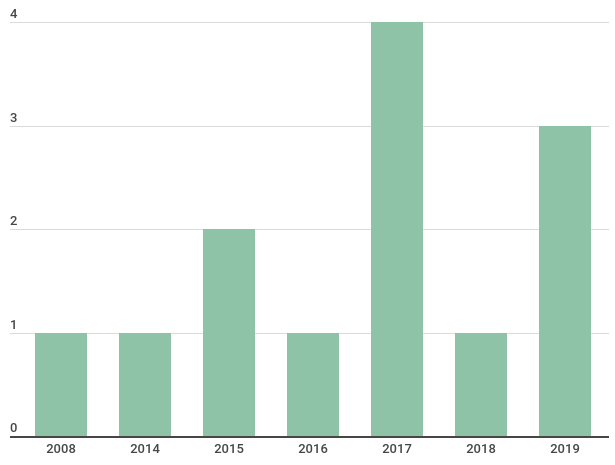
\includegraphics[width=\textwidth]{artigosA.png}
  %\caption{\label{fig:artigosA.png}Ano de publicação dos artigos Qualis A}
%\end{figure}
%
%\begin{figure}[!htb]
  %\centering
  %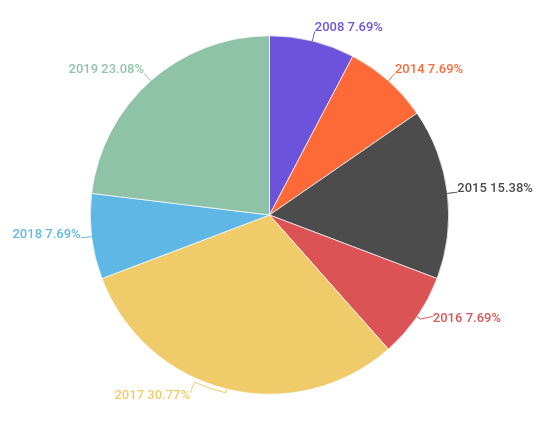
\includegraphics[width=\textwidth]{artigosA_pizza.png}
  %\caption{\label{fig:artigosA_pizza.png}Ano de publicação dos artigos Qualis A}
%\end{figure}


\section{Sensoreamento (camada de percepção)}\label{Sensoreamento do solo (camada de percepção)}

Tendo em vista a vasta variabilidade dos sensores utilizados nas diversas pesquisas apresentadas, agregamos os melhores resultados a cerca dos sensores.

\subsection{Umidade do solo}\label{Umidade do solo}

A literatura sobre a umidade do solo é muito extensa e está se desenvolvendo rapidamente, tornando difícil apresentar o estado da arte\cite{11} no que diz respeito à essa variável-chave, sendo essa definida pela água presente no solo\cite{11}, normalmente na parte superior, porém em diversos casos práticos pode-se obter o valor da umidade em diferentes profundidades, visando maior precisão e compreensão de outros fatores meteorológicos, como apresentado no trabalho de~\citeauthor{12}.

Segundo~\citeauthor{3}, os métodos mais aceitos para medição da umidade do solo são \textit{time domain reflectometry (TDR)} em português reflectometria no domínio do tempo, caso do sensor TDR CS616\cite{12}, e os métodos que medem a capacitância, sendo esses utilizados pela maioria dos sensores modernos.

Analisando esses sensores o autor supracitado\cite{3} realizou diversos testes alterando parâmetros como salinidade do solo, condutividade elétrica, temperatura entre outros, com os sensores EC-5 e ECH$_2$O-TE, chegando a seguinte conclusão, que após a devida calibração medições realizadas a uma frequência de 70 MHz obtém-se dados expressivos, sendo essa a frequência mais eficiente, pois acima dela o gasto energético  e eletrônico não resultam em maior precisão. Sendo assim para cada sensor deve ser achado a frequência ideal de medição na qual o custo é minimizado e a precisão é aumentada.

Esses sensores de umidade que medem a capacitância apesar de seguirem o mesmo princípio de funcionamento, podem variar muito de preço e precisão. Por exemplo, caso seja necessário uma elevada precisão bem como outros dados tais como salinidade e temperatura será utilizado um sensor mais caro como o utilizado por \citeauthor{12} para medições precisas o suficiente para agendar irrigação por gotejamento em estufas, tais medições foram feitas com 2 sensores Hydra probes, um a 15 cm de profundidade e outro medindo desses 15 cm até a superficie.

Como já comentado no parágrafo anterior os sensores variam muito de preço e funcionalidades. Sendo assim não existe um sensor perfeito ou universal para todo tipo de projeto, dessa maneira faz-se necessário que se avalie o orçamento bem como as funcionalidades e precisão exigidas, para auxiliar nisso é apresentada a tabela~\ref{sensores umidade}. Nessa tabela é apresentado o nome do sensor seguido de seu nível de precisão para 3 variáveis, a temperatura do solo, condutividade elétrica e umidade, por fim cita-se um trabalho no qual é utilizado o sensor.

\begin{savenotes}
\begin{table}[!htb]
  \centering
  \caption{Comparando sensores de umidade do solo.}
  \label{sensores umidade}
  \begin{tabular}{lllll}
    \hline
    \textbf{Sensor} & \textbf{Temp.}       & \textbf{Cond. E.} & \textbf{Umid.}  & \textbf{Autor}  \\ \hline
    Hydra Probe\footnote{Hydra Probe datasheet:~\url{http://overtechsolucoes.com.br/storage/datasheets/Hydra_Probe_II_Datasheet.pdf}}&$\pm~0,1$\textdegree~C&  $\pm~2\%$       & $\pm~0,03 \% $       & \citeauthor{12} \\
    ECH$_2$O\footnote{ECH$_2$O datasheet:~\url{https://sndl.ucmerced.edu/files/MHWG/Sensors_and_Loggers/Manuals/ECH2O_TE_TM.pdf}} & $\pm~1$\textdegree~C & $\pm~10 \%$       & $\pm~3\%$ & \citeauthor{3}  \\
    EC-5\footnote{EC-5 datasheet:~\url{http://www.bjsydz.com/data/Datasheet/EC-5.pdf}}&  X                   &  X                &  $\pm~2\%$   & \citeauthor{13} \\ \hline
  \end{tabular}
\end{table}
\end{savenotes}

\subsection{Temperatura e umidade do ambiente}\label{Temperatura e umidade do ambiente}

\subsubsection{LM35}\label{LM35}
Um sensor analógico de temperatura segundo seu fabricante (Texas Instruments Inc., TX, USA)\footnote{LM35 datasheet:~\url{https://www.ti.com/lit/ds/symlink/lm35.pdf}} é um dispositivo básico criado para medir a temperatura do ambiente, porém no caso da pesquisa de \citeauthor{9}, foi utilizado para medir a temperatura do solo, mostrando assim sua versatilidade.

Além de ser um sensor barato e de fácil acesso o LM35 é um dos sensores mais utilizados devido ao fato de produzir um output simples e diretamente relacionado a graus Celsius. Sua saída analógica tem uma certa voltagem que a cada 10 micro volts representam 1\textdegree~C, sendo assim 350 mV representam 35\textdegree~C.

%\subsubsection{DHT22}\label{DHT22}
%Utilizado por \citeauthor{7}~(SUNROM, Isanpur Ahmedabad, Gujarat, India)\footnote{DHT22 datasheet:~\url{https://www.sparkfun.com/datasheets/Sensors/Temperature/DHT22.pdf}}

%\subsubsection{DHT11}\label{DHT11}
%Utilizado por \citeauthor{13} para detectar condições desfavoráveis em vinhedos.\footnote{DHT11 datasheet:~\url{http://robocraft.ru/files/datasheet/DHT11.pdf}}

\subsubsection{DHT11 e DHT22}\label{DHT11 e DHT22}
Dois sensores muito parecidos, que leem tanto a umidade quanto a temperatura do ar, desenvolvidos por~(SUNROM, Isanpur Ahmedabad, Gujarat, India) o sensor DHT22\footnote{DHT22 datasheet:~\url{https://www.sparkfun.com/datasheets/Sensors/Temperature/DHT22.pdf}} apesar de mais caro possui maior precisão, $\pm 0,5$\textdegree~C, comparado aos 2 graus de precisão do DHT11, além de possuir maior faixa de valores de leitura e maior taxa de amostragem, por isso foi utilizado na pesquisa de \citeauthor{7}.

Já o DHT11\footnote{DHT11 datasheet:~\url{http://robocraft.ru/files/datasheet/DHT11.pdf}}, apesar de suas limitações supracitadas, conseguiu atender os requisitos de \citeauthor{13}, dessa maneira detectando condições desfavoráveis em vinhedos tradicionais do sul do Azerbaidjão.

\subsubsection{DS18B20}\label{DS18B20}
Um termômetro de ambiente desenvolvido pela empresa (Maxim Integrated, San Jose, CA, USA)\footnote{DS18B20 datasheet:~\url{https://pdf1.alldatasheet.com/datasheet-pdf/view/230838/DALLAS/DS18B20/+Q318W-VCvKlwudHXt.ICv+/datasheet.pdf}}, esse sensor foi utilizado na pesquisa de \citeauthor{9} devido a ser um sensor digital com uma precisão alta, $\pm~0,5$\textdegree~C

\subsubsection{SHT2x}\label{SHT2x}
Uma família de sensores de umidade da empresa (SENSIRION, Staefa ZH, Suíça)\footnote{SHT20 datasheet:~\url{https://www.sanatbazar.com/components/com_jshopping/files/demo_products/sensirion_SHT20.pdf}}, seu diferencial é que produz medições no padrão I$^2$C, permitindo assim múltiplos elementos (escravos), controlados pela mesma porta (SDA e SCL) de um controlador.

Apesar das vantagens de tal protocolo utilizado, pode ser difícil padronizar interfaces\cite{4}, principalmente considerando uma variedade de sensores.

\section{Rede (camada de comunicação)}\label{Rede (camada de comunicação)}

Atualmente são implementadas muitas redes de sensores sem fio (RSSF) para auxiliar a agricultura de precisão\cite{6}, sendo assim esses sensores necessitam de comunicação para exportar os dados coletados da maneira mais eficiente, gastando a menor quantidade de recursos de rede e energia\cite{5}. Essa seção abordará alguns dos principais protocolos que ligam dispositivos IOT, sendo eles\cite{5}, Bluetooth Low Energy (BluetoothSmart) e LoRaWAN\texttrademark, porém existem muitos outros como Zigbee, Sigfox, 3G/4G/5G, 6LoWPAN, entre outros, a escolha para determinado protocolo depende de diversos fatores tais como distância, custo energético, sendo assim exitem protocolos melhores para determinadas situações\cite{7}.

\subsection{Bluetooth Low Energy (BLE)}\label{Bluetooth Low Energy (BLE)}
\subsubsection{Definindo}\label{Definindo}
Assim como o Bluetooth tradicional o BLE é um sistema de comunicação via rádio, porém arquitetado para operar com pouco gasto de energia\cite{siteBluetooth}, Segundo o estudo de~\citeauthor{ble} chegando ao ponto de dispositivos que possuem baterias do tamanho de moedas operarem por meses. E segundo o site oficial do Bluetooth\cite{siteBluetooth} o gasto de energia do BLE é de 1\% a 50\% do Bluetooth clássico dependendo da aplicação.

\subsubsection{Vantagens e aplicações}\label{Vantagens e aplicações}
O BLE torna-se uma opção viável para comunicação de curta distancia pelo fato de operar com 3 canais\cite{ble} que buscam dispositivos próximos, restabelecendo a comunicação quando encontrados, apesar de possuir no total menos canais que o Bluetooth tradicional, cada canal possui a mesma frequência de transferência, 2.4 GHz, atingindo taxas de transmissão de até 1Mb/s\cite{5} em distâncias de até 100 metros\cite{5}. Essas e outras características tornam o Bluetooth Low Energy mais simples e econômico para transferências robustas de dados a curtas distâncias\cite{ble}.
% Mostrar o caso de alguém que usa ble aqui no final

\subsection{LoRaWAN~\texttrademark}\label{LoRaWAN}
Antes de definirmos o que é LoRaWAN~\texttrademark, suas especificações e aplicações, faz-se necessário que entenda-se o que é LORA~\textregistered.

\subsubsection{Definindo LORA~\textregistered}\label{Definindo LORA}
É a parte física da implementação, formada por diversas antenas\cite{siteLorawan}, que se comunicam utilizando a tecnologia de \textit{Chirp Spread Spectrum}\cite{lorawan} uma tecnologia de comunicação militar adaptada para uso comercial de mais baixo custo\cite{siteLorawan} tais antenas possuem alcance de até 15 km em áreas rurais % no texto ta escrito sub urbanas (suburban)
\cite{limiteLora}, bem como uma taxa média de duração de bateria de 10 anos\cite{limiteLora}.

\subsubsection{Definindo LoRaWAN~\texttrademark}\label{Definindo LoRaWAN}

É o protocolo de comunicação que utiliza a rede Lora~\textregistered\cite{siteLorawan}, arquitetado especificamente para atender aos requisitos da agricultura de precisão, onde muitos sensores geram dados os quais precisam ser analisados\cite{lorawan}. Os dados coletados chegam ao servidor através de uma rede com arquitetura de estrela\cite{siteLorawan}, dessa forma a complexidade fica no lado do servidor não no nó, assim reduzindo o custo energético.

Visando atender aplicações diferentes que demandam recursos diferentes esse sistema possui classes\cite{siteLorawan}, sendo elas:
\begin{itemize}
	\item \textbf{Classe A}: Mais econômica energeticamente, suportada por todos os dispositivos.
	\item \textbf{Classe B}: Menos econômica energeticamente que a classe A, porém mais econômica que a C, tem latência controlada pelo \textit{downlink}.
	\item \textbf{Classe C}: Menos econômica energeticamente, não possui latência na comunicação, o dispositivo não ``dorme'' e fica escutando continuamente.
\end{itemize}

\subsubsection{Vantagens}\label{Vantagens}
Apesar de não ser a solução mais barata, comparado ao BLE da seção~\ref{Bluetooth Low Energy (BLE)}, o custo para implantar a infraestrutura tem bom custo benefício\cite{siteLorawan}, além do fato de tanto o Lora\textregistered~quanto o LoRaWAN\texttrademark~possuírem código aberto\footnote{Github do LoRa:~\url{https://github.com/Lora-net}}~\footnote{Github do LoRaWAN:~\url{https://github.com/LoraWan}}, reduzindo assim seu custo. Comparando às outras opções de mercado possui um bom alcance, uma boa duração de bateria e principalmente é prático para inserção de novos nós e na comunicação com diferentes plataformas\cite{lorawan}.

%\cite{loraGithub}\cite{lorawanGithub}


\section{Plataformas de tomada de decisão (camada de aplicação)}\label{Plataformas de tomada de decisão}

Apesar de existir iniciativas que visem plataformas de tomada de decisão mais universais e interoperáveis tais como o mySense\cite{7}(software livre) e o SenseTube\cite{6}(software proprietário), a maioria das plataformas de tomada de decisão abaixo tendem a resolver um único problema específico ou servem apenas para pesquisas.

%que facilitem a criação de interfaces com o usuário final bem como a calibração de sensores

%Explicar como cada plataforma de tomada de decisão é diferente e cada autor decide implementar da sua maneira, apesar de ter esforços para padronizações\cite{6}



De acordo com a pesquisa de~\citeauthor{1} até onde sabe-se no ano de~\citeyear{1} não havia nenhuma plataforma ou \textit{framework} que baseando-se na temperatura do solo fornecesse dados dinâmicos para informar em tempo real decisões agronômicas dependentes do solo, tal como momento do plantio, irrigação entre outros.

Considerando essa lacuna do conhecimento, desenvolveu-se uma ferramenta de suporte à decisão da temperatura do solo, ``\textit{temperature decision support tool}'', seguindo uma metodologia de cinco passos:
\begin{enumerate}
  \item Comparação dos dados climáticos e ambientais, conseguindo a variabilidade em larga escala da temperatura do solo.

  \item Comparação das temperaturas médias em séries históricas.
  \item Comparar variáveis preditoras de clima com as medições realizadas, obtendo previsões.
  \item Transformar o sistema para funcionar em tempo real.
  \item Investigações a longo prazo.
\end{enumerate}

Com o objetivo de aumentar a precisão utiliza-se nove variáveis preditoras de clima, sendo elas: temperatura máxima, radiação diária, diferença entre temperatura máxima e mínima, taxa pluviométrica, latitude, elevação, conteúdo de água do solo, difusão térmica do solo, dia do ano.

Este sistema foi desenvolvido em Shiny (R), e possui uma alta taxa de predição de 92\% de validação cruzada R$_{2}$, RMSE = 1,91, tendência percentual = $-$ 0,01.
Com essas taxas de predição pode-se auxiliar os agricultores de algodão a realizarem o plantio no momento certo, classificando o solo como ``bom'' após três dias com temperaturas acima de 14\textdegree C, dessa maneira após utilizar dados de variáveis preditoras supracitadas recomenda-se ou não o plantio.

Outro sistema de apoio à decisão desenvolvido por~\citeauthor{2}, com o objetivo de monitorar vinhedos para encontrar e tratar ``míldio'' (mofo).
O míldio é uma doença fúngica causada pela \textit{plasmopara viticola oomycete}, doença essa que causa muito prejuízo nas vinícolas\cite{2}. Doença essa muito estudada, sendo assim nessa pesquisa baseando-se nos modelos já existentes de detecção a acompanhamento do fungo, buscou-se a automatização dos mesmos.

O principal modelo utilizado para descobrir qual o momento mais propício de aparecimento do míldio foi o de Goidanich\cite{detectando_milidio}, também chamado de ``regra dos três dez'' pois quando a temperatura média ultrapassa 10\textdegree C, a germinação ultrapassa os 10 cm e o volume de chuva superior a 10 mm, este é o momento propício para uma primeira contaminação da vinha.
Sabendo desses dados expostos por Goidanich\cite{detectando_milidio} percebe-se a necessidade de monitorar três fenômenos, sendo eles: temperatura, umidade e índice pluviométrico, sendo assim precisando de três sensores.

Para desenvolver essa plataforma o autor utilizou o sistema ``\textit{Sense Our Environment}'' (SEnviro), uma plataforma que utilizando-se de software e hardware livres visa baixar o custo e aumentar a eficiência energética dos sensores\cite{2}. O SEnviro contém suas funcionalidades melhor explicado em outra pesquisa\cite{SEnviro} e como já citado nessa seção possui todos os códigos fonte disponível ao público no github\footnote{Github do grupo de pesquisa:~\url{https://github.com/GeoTecINIT/}}
%\cite{SEnviro_Github}.


Com a estação concluída iniciou-se os testes, detectando em 96,9\% de maneira precisa em que houve o alerta de infecções. Através disso, os agricultores puderam aplicar o tratamento de controle de praga apenas quando necessário, reduzindo assim a quantidade de produtos químicos no solo, a quantidade de horas gastas para verificação e correção de doenças dentro do vinhedo bem como os custos da plantação.

\section{Considerações finais}
Em se tratando de agricultura de precisão, percebe-se neste trabalho que a internet das coisas, em suas diversas camadas, deve melhorar a coleta e interpretação de variáveis relevantes, dessa maneira diminuindo custos e aumentando a produtividade.

Observando cada um dos níveis dos sistemas \textit{IOT}, tem-se que, existem muitos sensores diferentes para medir determinados elementos, cada sensor com suas próprias especificações, estratégias de medição, vantagens, desvantagens, dessa maneira na seção~\ref{Sensoreamento do solo (camada de percepção)}, tentou-se listar os sensores mais benéficos, baseando-se no seu uso nas últimas aplicações de ponta, apesar do uso ou não de um sensor depender muitos fatores e não existir um único sensor que seja o melhor para qualquer tipo de uso.

Outrossim, no que se refere a sistemas de comunicação observou-se na seção~\ref{Rede (camada de comunicação)}, duas principais tecnologias a LoRaWAN\texttrademark~e o BLE, analisando assim comunicação tanto em curtas como em longas distâncias.

Por fim a seção~\ref{Plataformas de tomada de decisão} analisa aplicações que a partir dos dados coletados nas outras camadas, auxiliam o proprietário de área rural a tomar suas decisões. Nesse nível o software é muito específico a cada cenário, porém observa-se o uso de tecnologias que permitem a portabilidade para múltiplos sistemas e máquinas.


% ----------------------------------------------------------
% ELEMENTOS PÓS-TEXTUAIS
% ----------------------------------------------------------
\postextual

% ----------------------------------------------------------
% Referências bibliográficas
% ----------------------------------------------------------
%\cleardoublepage
\bibliography{ref}

\end{document}
